\documentclass{article}
\usepackage{amsmath}
\usepackage{xcolor}
\usepackage{amsthm}
\usepackage{graphicx}
\usepackage{hyperref}

\theoremstyle{definition}
\newtheorem{eg}{Example}[section]

\title{Traffic Scheduling}
\author{Jeroen van Riel}
\date{Oktober 2023}

\begin{document}

\maketitle

\section{Preliminaries}

\subsection{Single Machine Scheduling}

% total completion time and SPT rule
Suppose we have $n$ jobs that need processing on a single machine. The time
required for each job $j \in \{1, \dots, n\}$ is called the \textit{processing
  time} $p_{j}$. Once started, jobs may not be \textit{preempted}. In order to
obtain a valid \textit{schedule}, we need to determine the start time $y_{j}$
for each job $j$, such that at most one job is processing on the machine at all
times. Let $C_{j} = y_{j} + p_{j}$ denote the \textit{completion time} of job
$j$. Our objective is to minimize the \textit{total completion time}
$C_{1} + \dots + C_{n}$. By means of an \textit{interchange argument}, it can be
easily shown that an optimal solution is given by sorting the jobs according to
increasing processing times, which is known as the Shortest Processing Time
first (SPT) rule.

% release dates and non-delay schedules
Now suppose that job $j$ becomes available at its \textit{release date} $r_{j}$,
then a valid schedule requires $y_{j} \geq r_{j}$. It is not difficult to see
that non-uniform release dates may require us to introduce \textit{idle time} to
obtain an optimal schedule. For example, consider $n=2$ jobs with processing
times $p_{1}=2, p_{2}=1$ and release dates $r_{1}=0, r_{2}=\epsilon > 0$.
Processing job 1 before job 2 results in a schedule with total completion time
$\sum C_{j} = 2 + 3 = 5$. However, scheduling job 2 first requires us to
introduce $\epsilon$ idle time, but has a better total completion time of
$\sum C_{j} = (\epsilon + 1) + (\epsilon + 1 + 2) = 4 + 2 \epsilon$. Schedules
without idle time are called \textit{non-delay}.

% job families, precedence chains
Next, we consider \textit{precedence constraints} between jobs. Suppose that job
$j$ needs to be processed before job $l$, denoted as $j \rightarrow{} l$, then
we simply require that $y_{l} \geq C_{j}$ in any feasible schedule. In
particular, we may consider \textit{chains} of precedence constraints. Let
$J_{1}, \dots, J_{k}$ be a partition of jobs into $k$ non-empty families. For
each family, we require that their jobs $J_{l} = \{ j_{1}, \dots, j_{n_{l}}\}$
are processed in the order
$j_{1} \rightarrow{} j_{2} \rightarrow{} \dots \rightarrow{} j_{n_{l}}$, without
loss of generality. Note that the order between jobs from different families is
unspecified, which means that chains may be \textit{merged} arbitrarily.

% setup (switch-over) times
When job $j$ is directly followed by job $l$, we might want to introduce
\textit{sequence-dependent setup time} $s_{jl}$, by requiring that
$y_{l} \geq C_{j} + s_{jl}$. For our purposes, we will only consider setup times
depending on the family to which jobs belong. Formally, for any pair of jobs
$j_{1} \in J_{l_{1}}$ and $j_{2} \in J_{l_{2}}$ belonging to distinct families, we
require that either
\begin{align*}
y_{j_{2}} \geq C_{j_{1}} + s_{l_{1},l_{2}} ,
\end{align*}
is satisfied or
\begin{align*}
y_{j_{1}} \geq C_{j_{2}} + s_{l_{2},l_{1}} .
\end{align*}

\subsection{Single Intersection Scheduling}

We are interested in the task of assigning arriving vehicles to a time slot on a
single intersection. Using the modelling ingredients introduced above, we can
now pose this task as a scheduling problem. Let vehicles be represented by jobs.
We will refer to $y_{j}$ as the \textit{crossing time}, since it represents the
time at which the vehicle starts crossing the intersection, which is modelled by
the single machine. The time it takes before the next vehicle can enter the
intersection is modelled by the processing time $p_{j}$. The earliest possible
crossing time of a vehicle is modelled by its release date $r_{j}$. All vehicles
that arrive to the intersection from the same lane belong to the same family. We
assume that vehicles are driving on single-lane roads, which means that we do
not allow \textit{overtaking}. We model this by introducing chain precedence
constraints based on the order of arrival (release dates). To guarantee safety,
we require a setup time $s_{l_{1},l_{2}}$ between vehicles coming from different
lanes. As the optimization objective, we consider the total completion time,
since this is equivalent to minimizing the total delay experienced by all
vehicles.

% complexity
The problem of minimizing the total completion time with release dates (written
as $1 | r_{j} | \sum C_{j}$ in the three-field notation
\cite{grahamOptimizationApproximationDeterministic1979}) has been long known to
be NP-hard \cite{lenstraComplexityMachineScheduling1977}, so there is no hope in
finding a polynomial algorithm for our more general problem unless
$\mathcal{P} = \mathcal{NP}$. Therefore, we must resort to exhaustive
branch-and-bound methods or heuristics.

% assumptions
From here on, we will assume uniform processing time $p$ and uniform setup time
$s$, which is accurate enough to model vehicles that cross the intersection
without turning. For each job family $J = \{ 1, \dots, n \}$, observe that we
may assume that $r_{i} = \max\{ r_{i}, r_{i-1} + p \}$, without loss of
generality, because of the chain precedence constraints. Before discussing
solution methods, let us first consider some simple examples.

% examples
\begin{eg}
  Consider the situation with $J_{1} = \{ 1 \}, J_{2} = \{ 2 \}$. When both
  vehicles have the same release dates $r_{1} = r_{2} = r$, the order in which
  they cross the intersection does not influence the optimal total completion
  time of $\sum C_{j} = p + (p + S + p) = 3p + S$. Now, assume that vehicle 1
  has a earlier release date, then it is easily seen that an optimal schedule
  requires vehicle 1 to go first.
\end{eg}
%
\begin{eg}
  \label{example2}
  Consider the situation with $J_{1} = \{ 1 \}, J_{2} = \{ 2, 3 \}$. We are
  interested in how the release dates influence the order of the jobs in an
  optimal schedule. We assume that $r_{3} = r_{2} + p$. Suppose $r_{1} = r_{2}$,
  then we see that $2, 3, 1$ is optimal, which resembles some sort of ``longest
  chain first'' rule (\textit{\color{blue} relate this to Algorithm 3.1.4 of
    Pinedo}). Now assume that $r_{2} < r_{1} + p + s$, otherwise $1, 2, 3$ is
  simply optimal, because there is no \textit{conflict} between the two lanes
  (\textit{\color{blue}we will make this more precise later}). Furthermore, set
  $r_{1} = 0$, without loss of generality. We compare the sequence $1, 2, 3$
  with $2, 3, 1$. The first has optimal
  $\sum C_{j} = p + (p+s+p) + (p+s+p+p) = 6p + 2s$, while the second sequence
  has optimal
  $\sum C_{j} = (r_{2} + p) + (r_{2} + p + p) + (r_{2} + p + p + s + p) = 3 r_{2} + 6p + s$.
  Therefore, we conclude that the first sequence is optimal if and only if
  \begin{align*}
    r_{2} >= s/3 ,
  \end{align*}
  which roughly means that the ``longest chain first'' rule becomes optimal
  whenever the release dates are ``close enough''.
\end{eg}

\begin{figure}
  \centering
  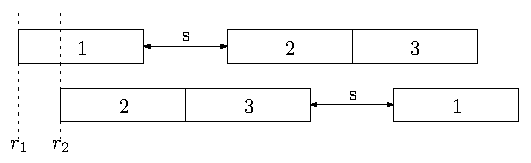
\includegraphics{123.pdf}
  \caption{Illustration of the two possible sequences in Example~\ref{example2}.}
  \label{fig:example2}
\end{figure}



\subsection{Branch-and-Bound}

Formulate the problem as a MIP and solve using branch-and-bound. Argue that
imposing maximum vehicle delay allows us to limit the set of disjunctions that
we need to consider.

\vspace{0.5em}
\noindent
\textit{\color{blue}lazy row generation}\\
\textit{\color{blue}define conflicts}


\subsection{Insertion Heuristic}

We propose a heuristic that constructs a schedule by considering the vehicles in
order of arrival and iteratively inserting each next vehicle in the current
partial schedule.


\section{Traffic Scheduling in Networks}

\subsection{Job Shop Scheduling}

This section shortly introduces the classical \textit{job shop} scheduling
problem. Assume there are $m$ machines and $n$ jobs. A job $j$ consists of
exactly $m$ operations, one for each of the machines. We let $(i,j)$ denote the
operation of job $j$ that needs to be processed on machine $i$. The time
required for processing operation $(i,j)$ is denoted by $p_{ij}$. The operations
of a job need to be executed in a fixed given order, which may be different
among jobs, and an operation may only start once its predecessor has completed
processing. Each machine can process at most one operation at the same time and,
once started, operations cannot be preempted.

Let the set of all operations be denoted by $N$. Furthermore, we encode the job
routes by defining the set $A$ of precedence constraints
$(i,j) \xrightarrow{} (k,j)$. Let $y_{ij}$ denote the start of operation
$(i,j)$. The completion time of job $j$ is defined as
$C_{j} := y_{lj} + p_{lj}$, where $l$ is the last machine on which $j$ must be
processed. A valid schedule is given by setting values for $y_{ij}$ such that
the above requirements are met. There are various measures for how \textit{good}
a given schedule is. For the purpose of this example, let us consider the
well-known makespan objective $C_{\text{max}} := \max_{j} C_{j}$, which is often
related to efficient use of the available machines. Minimizing the makespan can
now be formulated as a Mixed-Integer Program (MIP) as follows:
%
\begin{align*}
  \text{minimize } C_{\text{max}} \\
  y_{ij} + p_{ij} &\leq y_{kj}  & \text{ for all } (i,j) \xrightarrow{} (k,j) \in A \\
  y_{il} + p_{il} &\leq  y_{ij} \text{ or } y_{ij} + p_{ij} \leq y_{il}  & \text{ for all } (i,l) \text{ and } (i,j), i =1, \dots,m \\
  y_{ij} + p_{ij} &\leq C_{\text{max}} & \text{ for all } (i,j) \in N \\
  y_{ij} &\geq 0 & \text{ for all } (i,j) \in N
\end{align*}
%
The first set of constraints enforce the order of operations belonging to the
same job. The second set of constraints are called \textit{disjunctive}, because
they model that we need to choose between jobs $j$ and $l$ to be scheduled first
on machine $i$. The next constraints are used to define the makespan and the
last line enforces non-negative start times.


\subsection{MIP Formulation}
% TODO: introduce multiple lanes, opposing lanes on the same arc and consider
% multiple phases at intersections
% TODO: use ``arc'' instead of ``arc''
We now turn to vehicles traveling through a network of intersections. The
network may be thought of as a weighted directed graph $G=(V,E)$, with nodes and
arcs representing intersections and roads, respectively. \textbf{For now, we
  assume that the graph is acyclic}. Let $d(x,y)$ be defined as the
\textit{distance} between nodes $x$ and $y$. We assume there are no nodes of
degree two, since their two incident arcs $(x,y)$ and $(y,z)$ could be merged
into one arc $(x,z)$ with $d(x,z) = d(x,y) + d(y,z)$, without loss of
expressiveness. Furthermore, we assume the graph is connected. Each node of
degree one is called an \textit{external node} and models the location where
vehicles enter (\textit{entrypoint}) or exit (\textit{exitpoint}) the network. A
node of degree at least three is called an \textit{internal node} and models an
intersection.

Each vehicle $j$ enters the network at some external node $s$ and follows a
predetermined sequence of arcs
$R = ((s,i_{1}), (i_{1},i_{2}), \dots, (i_{n-1},i_{n}), (i_{n},d))$ towards an
external node $d$ where it leaves the network. Vehicles are not able to overtake
each other when traveling on the same arc. We assume that arcs provide
infinite \textit{buffers} for vehicles, meaning that there is no limit on the
number of vehicles that are traveling on the same arc at the same time.
However, we impose a minimum time required to travel along an arc $(x,y)$. By
assuming uniform maximum speed among vehicles, $d(x,y)$ can be directly
interpreted as this minimum travel time.

Let $y(i,j)$ denote the time vehicle $j$ enters intersection $i$. Crossing an
intersection takes $p$ time per vehicle and at most one vehicle can cross an
intersection at the same time. When two consecutive vehicles crossing an
intersection originate from the same arc, they may pass immediately after each
other. However, when a vehicle $j_{1}$ that wants to cross comes from a
different arc than the vehicle $j_{0}$ that last crossed the intersection, we
require that there is at least a \textit{switch-over time} $S$ between the
moment $j_{0}$ leaves and the moment $j_{1}$ enters the intersection.

Assuming that arrival times and routes of all vehicles are fixed and given, our
task is to determine when individual vehicles should cross intersections by
setting values for $y(i,j)$. This problem is similar to job shop scheduling,
with intersections and vehicles now taking the roles of machines and jobs, and
can also be formulated as a MIP, as we will show below.

% lane order is main difference with job shop
The main difference with job shop scheduling is related to the ordering of
vehicles. In the job shop model, every order $o \in \sigma_{n}$ of jobs on a
machine $i$ was allowed. By assuming that vehicles cannot overtake each other,
we are limiting the valid orderings.
% define common path and merge point
Given two routes $R_{j}$ and $R_{l}$, we define a common path
$p=(i_{1},\dots,i_{L})$ as a substring of both routes. We refer to the first
node $i_{1}$ of a common path as a \textit{merge point}. The set of all common
paths is denoted by $P_{jl}$.

Consider a common path $p$ whose merge point $i_{1}$ is an external node.
In this case, $i_{1}$ must be the entrypoint of both vehicles.
% first merge point
That means that the order on $p$ is determined by the order or arrival.
Let $r_{j}$ denote the arrival time (called the \textit{release date} in
scheduling) of vehicle $j$.
If $r_{j} < r_{l}$, then we require that $j$ goes first, formally stated as
\begin{align*}
  y_{ij} + p_{ij} \leq y_{il} \text{ for all } i \in p.
\end{align*}

% internal merge points are conflicts
Now suppose that $j$ and $l$ have a mergepoint $i_{1} \in p$ that is not an
external node, then these vehicles approach $i_{1}$ from different arcs,
which means that we have what we will call a \textit{conflict} between $j$ and
$l$, because the scheduler must choose which vehicle crosses the intersection
first. Furthermore, the switch-over time should be respected at $i_{0}$.
Requiring that vehicle $j$ must cross first can be formally stated as
\begin{align*}
  y_{i_{1}j} + p_{i_{1}j} + S \leq y_{i_{1}l} \text{ and } y_{ij} + p_{ij} \leq y_{il} \text{ for all } i_{1} \neq i \in p .
\end{align*}

% introduce s-variables
In order to model the above decision making with a MIP, we introduce binary
decision variables $s_{i,j,l}$ to encode the relative order of $j$ and $l$ at some common
node $i \in p \in P_{jl}$. A value of zero corresponds to $j$ crossing first and
a value of one indicates that $l$ crosses first.
In the case of $i_{1}$ being an external node, we treat $s_{i,j,l}$ as a fixed
parameter of the MIP.
For each common path $p \in P_{jl}$, we must have
\begin{align*}
s_{i_{1},j,l} = s_{i_{2},j,l} = \dots = s_{i_{L},j,l}.
\end{align*}

Let $N$ denote the set of operations like in the job shop example, but now pairs
correspond to vehicles and the intersections they encounter along their route.
Also similarly, let $A$ encode the route constraints of each vehicle. We use
$p_{1}$ to denote the merge point of path $p$. Let $P_{jl}^{e}$ denote all the
common paths that have an external merge point and let $P_{jl}$ denote the other
common paths. By implicitely letting the indices $j$ and $l$ run over all the
\textit{ordered pairs} of vehicles, we write
%
\begin{subequations}
\begin{align}
  \text{maximize } P(y) \\
  y_{ij} + p_{ij} + t_{ik} &\leq y_{kj}, & \text{ for all } (i,j) \xrightarrow{} (k,j) \in A, \\
  \label{1} y_{ij} + p_{ij} &\leq y_{il}, \text{ for all } i \in p, &\text{ for all } p \in P_{jl}^{e}, s_{p_{1}jl} = 1, \\
  \label{2} y_{p_{1}j} + p_{p_{1}j} + S &\leq y_{p_{1}l},  &\text{ for all } p \in P_{jl}, s_{p_{1}jl} = 1, \\
  \label{3} y_{ij} + p_{ij} &\leq y_{il}, \text{ for all } i \neq p_{1}, &\text{ for all } p \in P_{jl}, s_{p_{1}jl} = 1, \\
  y_{ij} &\geq 0, & \text{ for all } (i,j) \in N ,
  %
\end{align}
\end{subequations}
where $P(y)$ denotes some unspecified performance metric, leaving for now the
question of what it means for a schedule to be \textit{good}.
% explain how these 'if s=1' constraints can be implemented using the big-M technique
In order to solve this program using existing solvers, we use the well-known
\textit{big-M} method to encode which constraints from sets \eqref{1}, \eqref{2}
and \eqref{3} are active for specific values of the binary variables $s$.


\subsection{Structure in Network Schedules}

Before we start experimenting with the above problem (see if the MIP method
scales and later trying to learn policies with (MA)RL), we first should try to
find some common structural patterns in solutions or even some simple general
scheduling rules.

\begin{itemize}
  \item Study simple situations with the total completion time objective ($\sum C_{j}$), in which some kind of LPT rule holds. (\textit{TODO: explain why LPT-like schedules arise})
  \item Study tandem networks where the $\sum C_{j}$ objective causes platoon splitting due to some kind of ``propagation of delay costs''. (\textit{TODO: insert the example that I have})
  \item Can we study this ``delay cost propagation'' using some kind of dependency graph, e.g., by recording that delaying job A would require us to also delay job B, which would also require to delay C, etc.?
\end{itemize}

\subsection{Platoon Splitting}

In the single intersection case, platoon splitting is never necessary. So in
this context, platoon splitting can only become necessary from using a different
performance metric, e.g., one that takes into account fairness. Once we start
looking at the network-level interactions, however, we can show that platoon
splitting is sometimes necessary to obtain an optimal schedule. The main idea is
that delaying a job $j$ might require to also delay further downstream jobs.
Therefore, it might be cheaper overall to not delay $j$, but interrupt some
already running job $l$ instead.


\bibliography{references}
\bibliographystyle{ieeetr}

\end{document}
